\documentclass[a4paper,12pt]{article}
\usepackage{graphicx}
\usepackage[utf8]{inputenc}
\usepackage[T1]{fontenc}
\usepackage[italian]{babel}
\usepackage[a4paper,margin=2.5cm]{geometry}
\usepackage{enumitem}
\usepackage{hyperref}
\usepackage{float}

\title{Deliverable D1\\TrentoParking}
\author{}
\date{}

\begin{document}

\maketitle

\noindent \textbf{Numero del gruppo:} 12

\vspace{0.3cm}

\noindent \textbf{Componenti del gruppo:}
\begin{itemize}[leftmargin=1.2cm]
    \item David Dorobantu -- 234467
    \item Riccardo Gonzato -- 246476
    \item Matteo Sepa -- 243283
\end{itemize}

\section{Obiettivi del progetto}

L'obiettivo generale del progetto è supportare gli utenti nella ricerca di parcheggio nella città di Trento, riducendo il tempo perso nella ricerca casuale e fornendo una stima della disponibilità di parcheggi gratuiti e a pagamento in una zona selezionata.

\begin{itemize}[leftmargin=2.2cm]
    \item[\textbf{O1:}] Permettere all'utente di selezionare una zona di interesse sulla mappa della città di Trento.
    \item[\textbf{O2:}] Permettere all'utente di definire un raggio di ricerca rispetto alla zona selezionata.
    \item[\textbf{O3:}] Fornire una stima della disponibilità di parcheggi gratuiti e a pagamento nell'area considerata.
    \item[\textbf{O4:}] Supportare l'utente nella scelta tra ricerca di parcheggio gratuito e ricorso a parcheggi a pagamento, in base alle informazioni disponibili.
    \item[\textbf{O5:}] Integrare, quando disponibili, dati esterni relativi ai parcheggi monitorati e altri segnali contestuali utili a migliorare la qualità della stima.
    \item[\textbf{O6:}] Consentire agli utenti autenticati di inviare feedback sull'esito della ricerca del parcheggio, così da contribuire al miglioramento progressivo del sistema.
    \item[\textbf{O7:}] Contribuire indirettamente alla riduzione del traffico dovuto alla ricerca casuale di parcheggio, aiutando gli utenti a orientarsi verso aree più promettenti.
    \item[\textbf{O8:}] Incentivare la partecipazione attiva degli utenti autenticati tramite meccanismi di riconoscimento o premialità, utili a favorire il contributo collaborativo al sistema.
\end{itemize}

\section{Attori del sistema}

\subsection{Utenti}

\begin{itemize}
    \item \textbf{Utente non autenticato:} può accedere alle funzionalità di consultazione di base del sistema, come la visualizzazione della mappa, la selezione di una zona e la consultazione della stima della disponibilità di parcheggi gratuiti e a pagamento.

    \item \textbf{Utente autenticato/contributore:} oltre alle funzionalità dell'utente non autenticato, può inviare feedback sull'esito della ricerca di parcheggio e partecipare al miglioramento progressivo del sistema tramite contributi informativi.

    \item \textbf{Amministratore:} gestisce le configurazioni generali della piattaforma, supervisiona i dati utilizzati dal sistema e controlla eventuali meccanismi di incentivazione e contributo.
\end{itemize}

\subsection{Sistemi esterni}

\begin{itemize}
    \item \textbf{Sistema dati parcheggi del Comune di Trento:} fornisce dati esterni relativi ai parcheggi monitorati e ad altre informazioni utili al funzionamento del sistema.

    \item \textbf{Servizio cartografico:} fornisce le funzionalità di visualizzazione della mappa e di localizzazione delle aree di interesse.
\end{itemize}
\section{Requisiti funzionali per attore}

\subsection{Utente non autenticato}

\begin{itemize}[leftmargin=2cm]
    \item[\textbf{RF1:}] Il sistema deve permettere all'utente non autenticato di accedere alla mappa della città di Trento.
    \item[\textbf{RF2:}] Il sistema deve permettere all'utente non autenticato di selezionare una zona di interesse sulla mappa.
    \item[\textbf{RF3:}] Il sistema deve permettere all'utente non autenticato di definire un raggio di ricerca rispetto alla zona selezionata.
    \item[\textbf{RF4:}] Il sistema deve permettere all'utente non autenticato di visualizzare la stima della disponibilità di parcheggi gratuiti nell'area selezionata.
    \item[\textbf{RF5:}] Il sistema deve permettere all'utente non autenticato di visualizzare la stima della disponibilità di parcheggi a pagamento nell'area selezionata.
    \item[\textbf{RF6:}] Il sistema deve permettere all'utente non autenticato di confrontare la disponibilità stimata tra parcheggi gratuiti e parcheggi a pagamento.
    \item[\textbf{RF7:}] Il sistema deve permettere all'utente non autenticato di visualizzare eventuali aree vicine considerate più promettenti per la ricerca di parcheggio.
    \item[\textbf{RF8:}] Il sistema deve permettere all'utente non autenticato di visualizzare informazioni descrittive sul funzionamento del servizio e sul significato delle stime mostrate.
\end{itemize}

\subsection{Utente autenticato/contributore}

\begin{itemize}[leftmargin=2cm]
    \item[\textbf{RF9:}] Il sistema deve permettere all'utente autenticato di effettuare l'accesso alla piattaforma.
    \item[\textbf{RF10:}] Il sistema deve permettere all'utente autenticato di inviare un feedback sull'esito della ricerca di parcheggio in una determinata zona.
    \item[\textbf{RF11:}] Il sistema deve permettere all'utente autenticato di indicare se il parcheggio trovato \`e gratuito o a pagamento.
    \item[\textbf{RF12:}] Il sistema deve permettere all'utente autenticato di associare il feedback a una fascia oraria e a una zona di riferimento.
    \item[\textbf{RF13:}] Il sistema deve permettere all'utente autenticato di visualizzare lo storico dei feedback inviati.
    \item[\textbf{RF14:}] Il sistema deve permettere all'utente autenticato di ricevere un riconoscimento o una premialit\`a associata alla partecipazione attiva al sistema.
    \item[\textbf{RF15:}] Il sistema deve permettere all'utente autenticato di modificare o rimuovere un proprio feedback entro un intervallo di tempo definito.
\end{itemize}

\subsection{Amministratore}

\begin{itemize}[leftmargin=2cm]
    \item[\textbf{RF16:}] Il sistema deve permettere all'amministratore di accedere a un'area di gestione riservata.
    \item[\textbf{RF17:}] Il sistema deve permettere all'amministratore di configurare i parametri generali utilizzati per la generazione delle stime.
    \item[\textbf{RF18:}] Il sistema deve permettere all'amministratore di gestire le fonti dati esterne utilizzate dal sistema.
    \item[\textbf{RF19:}] Il sistema deve permettere all'amministratore di monitorare i feedback inviati dagli utenti autenticati.
    \item[\textbf{RF20:}] Il sistema deve permettere all'amministratore di gestire eventuali meccanismi di riconoscimento o premialit\`a previsti per gli utenti contributori.
\end{itemize}
\section{Requisiti non funzionali}

\begin{itemize}[leftmargin=2cm]
    \item[\textbf{RNF1:}] Il sistema deve fornire una risposta alla richiesta di stima della disponibilità di parcheggio in un tempo compatibile con un utilizzo interattivo dell'applicazione.
    
    \item[\textbf{RNF2:}] Il sistema deve essere accessibile da dispositivi desktop e mobili attraverso un'interfaccia web responsive.
    
    \item[\textbf{RNF3:}] L'interfaccia utente deve presentare in modo chiaro la distinzione tra parcheggi gratuiti e parcheggi a pagamento.
    
    \item[\textbf{RNF4:}] Il sistema deve garantire una navigazione semplice e comprensibile anche per utenti che utilizzano il servizio per la prima volta.
    
    \item[\textbf{RNF5:}] Il sistema deve proteggere i dati associati agli utenti autenticati e ai relativi feedback.
    
    \item[\textbf{RNF6:}] Il sistema deve garantire che solo gli utenti autenticati possano inviare, modificare o rimuovere feedback.
    
    \item[\textbf{RNF7:}] Il sistema deve essere progettato in modo da consentire l'integrazione di fonti dati esterne senza richiedere una completa riprogettazione della piattaforma.
    
    \item[\textbf{RNF8:}] Il sistema deve essere manutenibile, in modo da permettere aggiornamenti futuri relativi a nuove zone, nuove fonti dati o nuove logiche di stima.
    
    \item[\textbf{RNF9:}] Il sistema deve garantire coerenza nella visualizzazione delle informazioni mostrate sulla mappa e nelle stime associate alle aree selezionate.
    
    \item[\textbf{RNF10:}] Il sistema deve essere progettato in modo modulare, in modo da mantenere separate l'interfaccia utente, la gestione dei dati e la logica di elaborazione delle stime, così da facilitare manutenzione ed evoluzione futura.
\end{itemize}
\section{Use case diagrams e casi d'uso}

Il diagramma dei casi d'uso del sistema rappresenta le principali interazioni tra gli attori individuati e le funzionalità offerte dalla piattaforma TrentoParking. In particolare, il sistema consente agli utenti di consultare la mappa, selezionare un'area di interesse, visualizzare una stima della disponibilità di parcheggio e, nel caso degli utenti autenticati, contribuire con feedback. L'amministratore gestisce invece i dati e i parametri generali del sistema.

\begin{figure}[H]
    \centering
    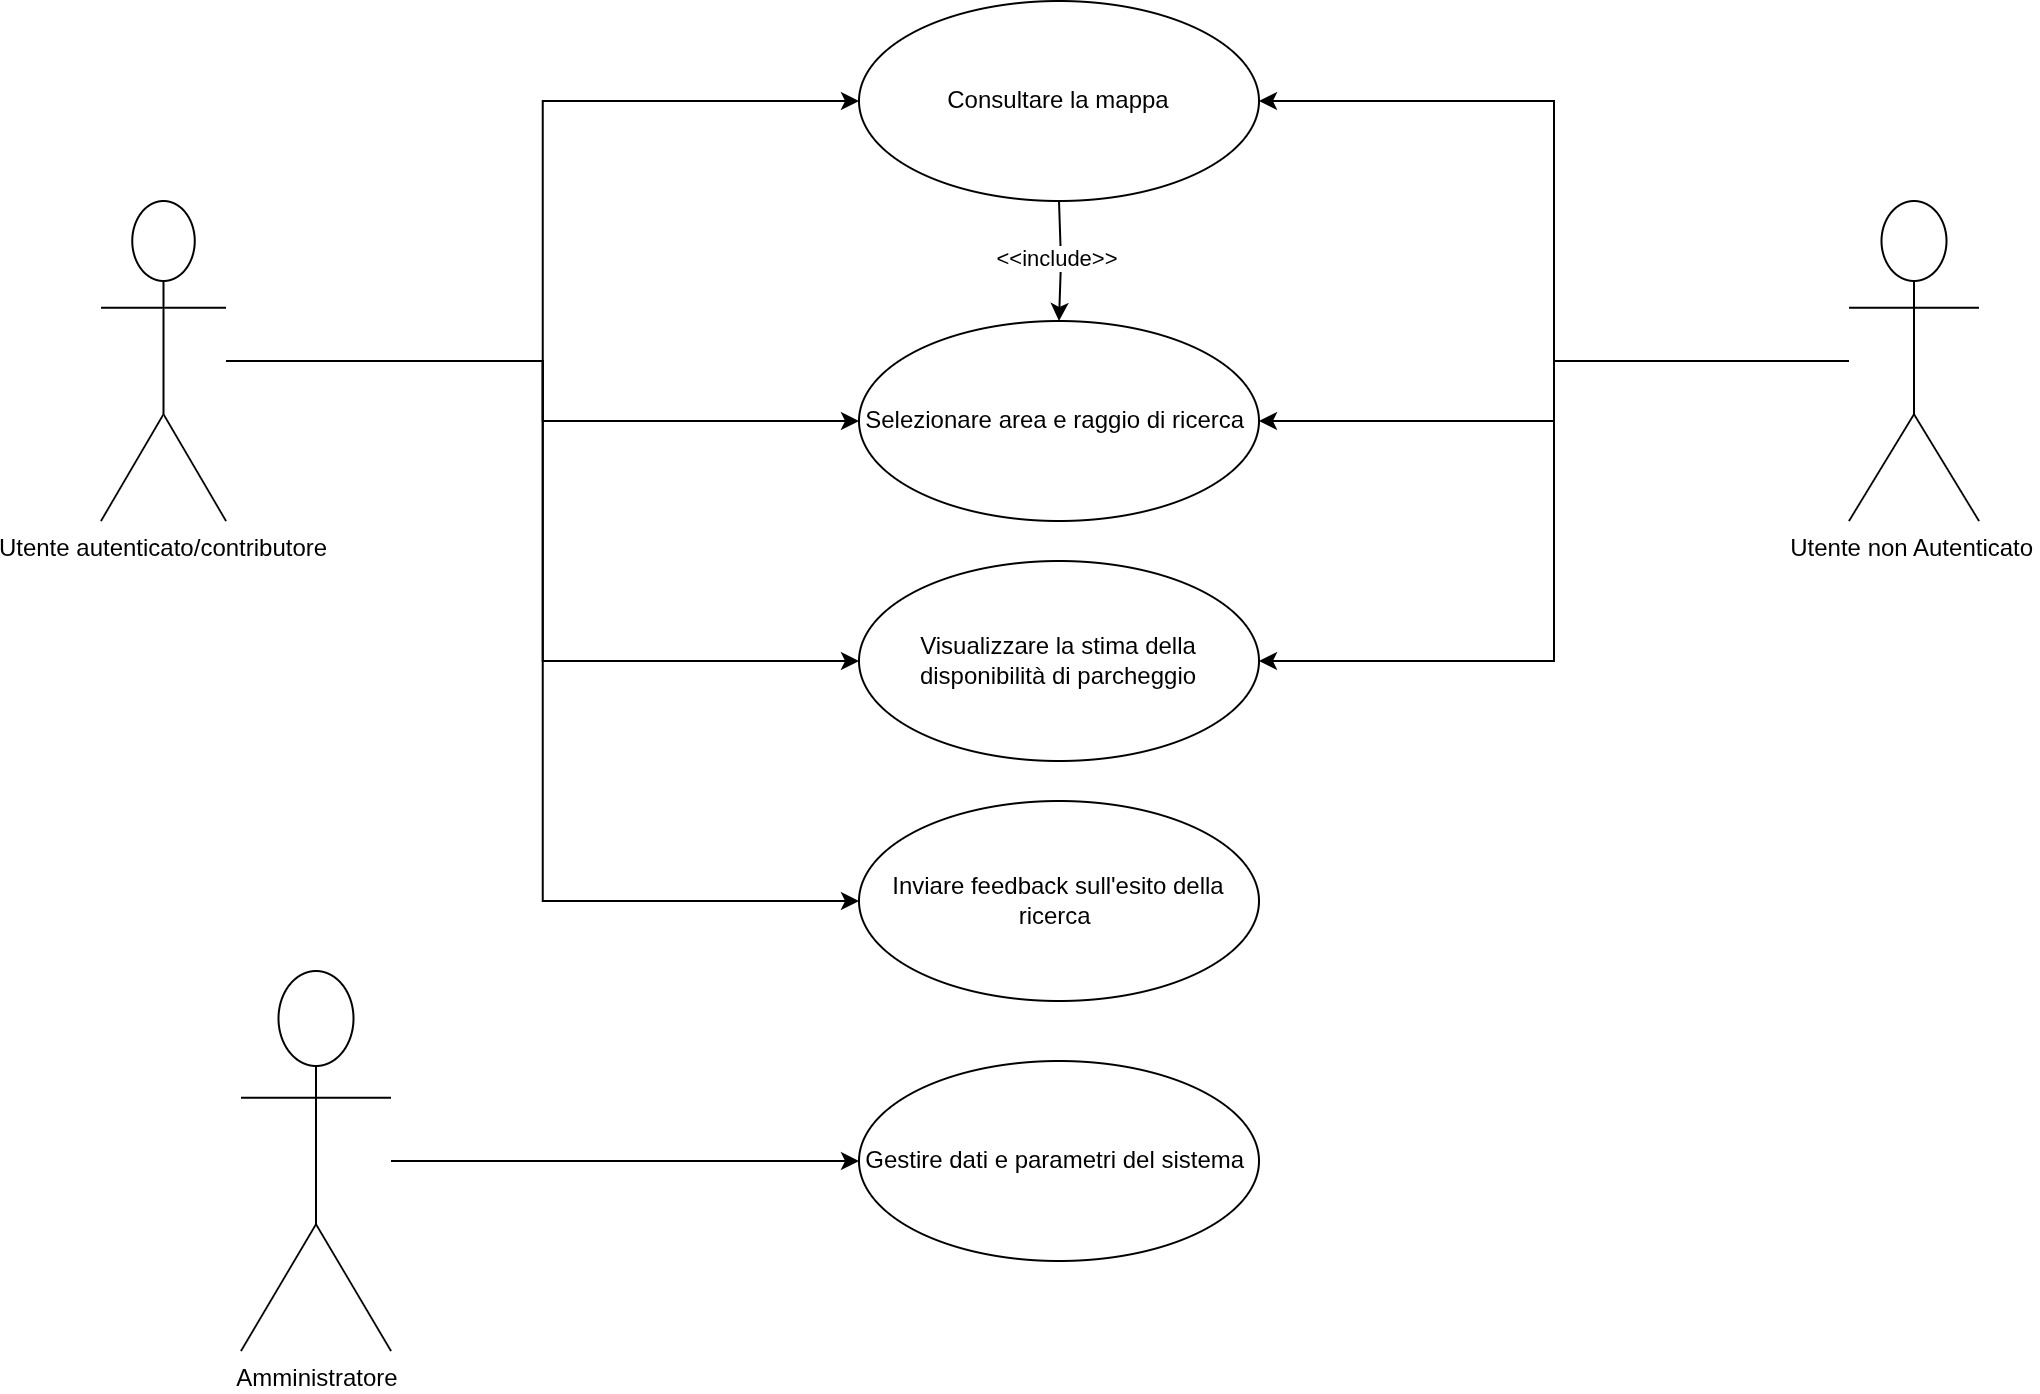
\includegraphics[width=\textwidth]{usecase.jpg}
    \caption{Diagramma dei casi d'uso di TrentoParking}
    \label{fig:usecase}
\end{figure}

I principali casi d'uso individuati per il sistema sono i seguenti:

\begin{itemize}
    \item \textbf{UC1:} Consultare la mappa
    \item \textbf{UC2:} Selezionare area e raggio di ricerca
    \item \textbf{UC3:} Visualizzare la stima della disponibilità di parcheggio
    \item \textbf{UC4:} Inviare feedback sull'esito della ricerca
    \item \textbf{UC5:} Gestire dati e parametri del sistema
\end{itemize}

\subsection*{UC1 -- Consultare la mappa}

\textbf{Attore principale:} Utente non autenticato, Utente autenticato/contributore

\textbf{Precondizioni:} Il sistema è disponibile e la mappa è accessibile.

\textbf{Descrizione:}  
L'utente accede al sistema e visualizza la mappa della città di Trento, con le informazioni di base necessarie alla consultazione del servizio.

\textbf{Flusso principale:}
\begin{enumerate}
    \item L'utente apre l'applicazione.
    \item Il sistema mostra la mappa della città di Trento.
    \item L'utente esplora la mappa per individuare la zona di interesse.
\end{enumerate}

\textbf{Postcondizioni:} L'utente ha accesso alla visualizzazione della mappa e può proseguire con la selezione dell'area di interesse.
\subsection*{UC2 -- Selezionare area e raggio di ricerca}

\textbf{Attore principale:} Utente non autenticato, Utente autenticato/contributore

\textbf{Precondizioni:} L'utente sta visualizzando la mappa del sistema.

\textbf{Descrizione:}  
L'utente seleziona una zona della città di Trento e definisce un raggio di ricerca entro il quale desidera ottenere una stima della disponibilità di parcheggio.

\textbf{Flusso principale:}
\begin{enumerate}
    \item L'utente seleziona una zona di interesse sulla mappa.
    \item Il sistema registra la posizione selezionata.
    \item L'utente imposta un raggio di ricerca.
    \item Il sistema acquisisce i parametri necessari alla ricerca.
\end{enumerate}

\textbf{Postcondizioni:} Il sistema dispone della zona e del raggio necessari per elaborare la stima di disponibilità.
\subsection*{UC3 -- Visualizzare la stima della disponibilità di parcheggio}

\textbf{Attore principale:} Utente non autenticato, Utente autenticato/contributore

\textbf{Precondizioni:} L'utente ha selezionato una zona e un raggio di ricerca.

\textbf{Descrizione:}  
Il sistema elabora le informazioni disponibili e mostra all'utente una stima della disponibilità di parcheggi gratuiti e a pagamento nell'area selezionata.

\textbf{Flusso principale:}
\begin{enumerate}
    \item L'utente conferma la richiesta di consultazione.
    \item Il sistema recupera i dati disponibili relativi all'area selezionata.
    \item Il sistema elabora la stima di disponibilità.
    \item Il sistema mostra la stima dei parcheggi gratuiti.
    \item Il sistema mostra la stima dei parcheggi a pagamento.
    \item Il sistema evidenzia eventuali aree vicine considerate più promettenti.
\end{enumerate}

\textbf{Postcondizioni:} L'utente visualizza la stima di disponibilità e può decidere come procedere nella ricerca del parcheggio.
\subsection*{UC4 -- Inviare feedback sull'esito della ricerca}

\textbf{Attore principale:} Utente autenticato/contributore

\textbf{Precondizioni:} L'utente ha effettuato l'accesso al sistema.

\textbf{Descrizione:}  
L'utente autenticato comunica al sistema l'esito della ricerca di parcheggio in una determinata zona, contribuendo al miglioramento progressivo delle stime.

\textbf{Flusso principale:}
\begin{enumerate}
    \item L'utente accede alla funzionalità di invio feedback.
    \item L'utente seleziona la zona di riferimento.
    \item L'utente indica l'esito della ricerca del parcheggio.
    \item L'utente specifica, se disponibile, la tipologia di parcheggio trovata.
    \item Il sistema registra il feedback associandolo all'utente e al contesto temporale.
\end{enumerate}

\textbf{Postcondizioni:} Il feedback viene memorizzato dal sistema e reso disponibile per successive elaborazioni.
\subsection*{UC5 -- Gestire dati e parametri del sistema}

\textbf{Attore principale:} Amministratore

\textbf{Precondizioni:} L'amministratore ha effettuato l'accesso all'area riservata.

\textbf{Descrizione:}  
L'amministratore configura i parametri generali del sistema e gestisce le fonti dati utilizzate per la generazione delle stime.

\textbf{Flusso principale:}
\begin{enumerate}
    \item L'amministratore accede all'area di gestione.
    \item Il sistema mostra le funzionalità amministrative disponibili.
    \item L'amministratore consulta o aggiorna i parametri del sistema.
    \item L'amministratore gestisce le fonti dati esterne.
    \item Il sistema salva le modifiche effettuate.
\end{enumerate}

\textbf{Postcondizioni:} I parametri e le fonti dati del sistema risultano aggiornati.
\end{document}